\def\duedate{\today}
\def\HWnum{4}
\documentclass[10pt,a4paper]{book}

% custom section formatting
\usepackage{titlesec}
\titleformat{\chapter}[display]
{\normalfont\Large\filcenter\sffamily}
{\titlerule[1pt]%
\vspace{1pt}%
\titlerule
\vspace{1pc}%
\LARGE\MakeUppercase{\chaptertitlename} \thechapter}
{1pc}
{\titlerule
\vspace{1pc}%
\Huge}

% appendix handling
\usepackage[toc,page]{appendix}
    
% encoding for file and font
\usepackage[utf8]{inputenc}
\usepackage[T1]{fontenc}

% math formatting/tools
\usepackage{amsmath}
\usepackage{amssymb}
\usepackage{mathtools}
\usepackage[arrowdel]{physics}

% unit formatting
\usepackage{siunitx}
\AtBeginDocument{\RenewCommandCopy\qty\SI}

% figure formatting/tools
\usepackage{graphicx}
\usepackage{float}
\usepackage{subcaption}
\usepackage{multirow}
\usepackage{import}
\usepackage{pdfpages}
\usepackage{transparent}
\usepackage{currfile}

\NewDocumentCommand\incfig{O{1} m}{
    \def\svgwidth{#1\textwidth}
    \import{./Figures/\currfiledir}{#2.pdf_tex}
}

\newcommand{\bef}{\begin{figure}[h!tb]\centering}
\newcommand{\eef}{\end{figure}}

\newcommand{\bet}{\begin{table}[h!tb]\centering}
\newcommand{\eet}{\end{table}}

% hyperlink references 
\usepackage{hyperref}
\hypersetup{
    colorlinks=true,
    linkcolor=blue,
    filecolor=magenta,
    urlcolor=cyan,
    pdftitle={Physics 1 Notes},
    pdfauthor={Richard Whitehill},
    pdfpagemode=FullScreen
}
\urlstyle{same}

\newcommand{\eref}[1]{Eq.~(\ref{eq:#1})}
\newcommand{\erefs}[2]{Eqs.~(\ref{eq:#1})--(\ref{eq:#2})}

\newcommand{\fref}[1]{Fig.~(\ref{fig:#1})}
\newcommand{\frefs}[2]{Fig.~(\ref{fig:#1})--(\ref{fig:#2})}

\newcommand{\aref}[1]{Appendix~(\ref{app:#1})}
\newcommand{\sref}[1]{Section~(\ref{sec:#1})}
\newcommand{\srefs}[2]{Sections~(\ref{sec:#1})-(\ref{sec:#2})}

\newcommand{\tref}[1]{Table~(\ref{tab:#1})}
\newcommand{\trefs}[2]{Table~(\ref{tab:#1})--(\ref{tab:#2})}

% tcolorbox formatting/definitions
\usepackage[most]{tcolorbox}
\usepackage{xcolor}
\usepackage{xifthen}
\usepackage{parskip}

\definecolor{peach}{rgb}{1.0,0.8,0.64}

\DeclareTColorBox[auto counter, number within=chapter]{defbox}{O{}}{
    enhanced,
    boxrule=0pt,
    frame hidden,
    borderline west={4pt}{0pt}{green!50!black},
    colback=green!5,
    before upper=\textbf{Definition \thetcbcounter \ifthenelse{\isempty{#1}}{}{: #1} \\ },
    sharp corners
}

\newcommand*{\eqbox}{\tcboxmath[
    enhanced,
    colback=black!10!white,
    colframe=black,
    sharp corners,
    size=fbox,
    boxsep=8pt,
    boxrule=1pt
]}

\newtcolorbox[auto counter, number within=chapter]{exbox}{
    parbox=false,
    breakable,
    enhanced,
    sharp corners,
    boxrule=1pt,
    colback=white,
    colframe=black,
    before upper= \textbf{Example \thetcbcounter:}\,,
    before lower= \textbf{Solution:}\,,
    segmentation hidden
}

\newtcolorbox{resbox}{
    enhanced,
    colback=black!10!white,
    colframe=black,
    boxrule=1pt,
    boxsep=0pt,
    top=2pt,
    ams nodisplayskip,
    sharp corners
}


\begin{document}

\prob{1}{

    Consider a potential problem in the half-space defined by $z \geq 0$, with Dirichlet boundary conditions on the plane $z = 0$ (and at infinity). \\[1pt]

(a) Write down the appropriate Green function $G(\va*{x},\va*{x}')$.

(b) If the potential on the plane $z = 0$ is specified to be $\Phi = V$ inside a circle of radius $a$ centered at the origin, and $\Phi = 0$ outside that circle, find an integral expression for the potential at the point $P$ specified in terms of cylindrical coordinates $(\rho,\phi,z)$.

(c) Show that, along the axis of the circle ($\rho = 0$), the potential is given by
\begin{eqnarray}
    \Phi = V \Big( 1 - \frac{z}{\sqrt{ a^2 + z^2}} \Big)
.\end{eqnarray}

(d) Show that at large distances ($\rho^2 + z^2 \gg a^2$) the potential can be expanded in a power series in $(\rho^2 + z^2)^{-1}$, and that the leading terms are
\begin{eqnarray}
    \Phi = \frac{Va^2}{2}\frac{z}{(\rho^2 + z^2)^{3/2}}  \Big[ 1 - \frac{3 a^2}{4 (\rho^2 + z^2)} + \frac{5( 3 \rho^2 a^2 + a^{4} )}{8( \rho^2 + z^2 )^2} + \ldots \Big]
.\end{eqnarray}
Verify that the results of parts (c) and (d) are consistent with each other in their common range of validity.

}

\sol{

(a) A Green's function satisfying
\begin{eqnarray}
    \laplacian G(\va*{x},\va*{x}') = -4 \pi \delta(\va*{x} - \va*{x}')
\end{eqnarray}
is $G(\va*{x},\va*{x}') = |\va*{x} - \va*{x}'|^{-1}$.
Now, we must find a Green's function satisfying Dirichlet boundary conditions on the $xy$-plane.
That is, we take $G \rightarrow G + F$, where $F$ solves Laplace's equation (in the half-space where $z \geq 0$) and $G + F$ satisfies the boundary condition $\Phi = 0$ when $z = 0$.
Such a choice is
\begin{eqnarray}
    \eqbox{ G(\va*{x},\va*{x}') = \frac{1}{|\va*{x}' - \va*{x}|} - \frac{1}{|\va*{x}' - \va*{y}|} }
,\end{eqnarray}
where $\va*{y}$ is $\va*{x}$ translated over the $xy$-plane (i.e. $z \rightarrow -z$ for $\va*{y}$).
It is clear then that the second term satisfies Laplaces equation for $z \geq 0$ and that the sum of these two functions is identically zero on the $xy$-plane.

(b) If we have the potential on the plane
\begin{eqnarray}
    \Phi(x,y,z = 0) = \begin{cases}
        V & x^2 + y^2 \leq a^2 \\
        0 & {\rm otherwise}
    ,\end{cases}
\end{eqnarray}
we can write the potential for $z \geq 0$ as
\begin{eqnarray}
    \Phi = \frac{1}{4 \pi \epsilon_0} \int_{V} \dd[3]{\va*{x}'} G(\va*{x},\va*{x}') \rho(\va*{x}') - \frac{1}{4 \pi} \int_{S} \dd{S'} \Phi(\va*{x}') \pdv{G(\va*{x},\va*{x}')}{n'}
.\end{eqnarray}
Observe that the first term is zero since there is no charge.
The second integral is over the circular surface of radius $a$ in the $xy$ plane such that
\begin{eqnarray}
    \eqbox{
    \begin{aligned}
        \Phi &= -\frac{V}{4 \pi} \int_{0}^{a} \int_{0}^{2\pi} \dd{\rho'} \dd{\phi'} \rho' \Big( - \pdv{G}{z'} \Big) \\
        &= \frac{V}{4 \pi} \int_{0}^{a} \int_{0}^{2 \pi} \dd{\rho'} \dd{\phi'} \rho' \frac{2z}{[ (x' - x)^2 + (y' - y)^2 + z^2 ]^{3/2}} \\
        &= \frac{V z}{2 \pi} \int_{0}^{a} \int_{0}^{2 \pi} \dd{\rho'} \dd{\phi'} \frac{\rho'}{[(\rho'\cos{\phi'} - \rho \cos{\phi})^2 + (\rho' \sin{\phi'} - \rho \sin{\phi})^2 + z^2]^{3/2}} \\
        &= \frac{Vz}{2 \pi} \int_{0}^{a} \int_{0}^{2\pi} \dd{\rho'} \dd{\phi'} \frac{\rho'}{[ \rho'^2 + \rho^2 - 2 \rho' \rho \cos{(\phi' - \phi)} + z^2 ]^{3/2}}
    .\end{aligned}
}
\end{eqnarray}
At this point, this is all we can do in full analytic generality.

(c) We consider a special case along the $z$ axis such that $\rho = 0$, which causes the previous expression to simply as
\begin{eqnarray}
    \eqbox{
    \begin{aligned}
        \Phi &= \frac{V z}{2 \pi} \int_{0}^{a} \int_{0}^{2 \pi} \dd{\rho'} \dd{\phi'} \frac{\rho'}{(\rho'^2 + z^2)^{3/2}} = V z \int_{0}^{a} \frac{\rho' \dd{\rho'}}{(\rho'^2 + z^2)^{3/2}} \\
        &= Vz \Bigg[ \frac{1}{z} - \frac{1}{\sqrt{z^2 + a^2}} \Bigg] = V \Bigg[ 1 - \frac{z}{\sqrt{z^2 + a^2}} \Bigg]
    \end{aligned}
    }
\end{eqnarray}
as desired.

(d) There is another case in which we can do the integration, which is when we are far away from circular surface with radius $a$ in the $xy$-plane (i.e. $\rho^2 + z^2 \gg a^2$).
In this case, we can write
\begin{eqnarray}
    \label{eq:prob1c}
    \Phi = \frac{V z}{2 \pi} \frac{1}{(\rho^2 + z^2)^{3/2}} \int_{0}^{a} \int_{0}^{2 \pi} \dd{\rho'} \dd{\phi'} \rho' \Bigg[ 1 + \frac{\rho'^2 - 2 \rho' \rho \cos{(\phi' - \phi)}}{\rho^2 + z^2} \Bigg]^{-3/2}
.\end{eqnarray}
Notice that the expression in brackets is of the form $(1 + x)^{n} = 1 + nx + [n(n-1)/2!] x^2 + \ldots $, so the double integral becomes
\begin{eqnarray}
    \begin{aligned}
        \int_{0}^{a} \int_{0}^{2 \pi} \dd{\rho'} \dd{\phi'} \rho' &\Bigg[ 1  - \frac{3}{2} \Big( \frac{\rho'^2 - 2 \rho' \rho \cos{(\phi' - \phi)}}{\rho^2 + z^2} \Big) + \frac{15}{8} \Big( \frac{\rho'^2 - 2 \rho' \rho \cos{(\phi' - \phi)}}{\rho^2 + z^2} \Big)^2 + \ldots \Bigg] \\
        &= \pi a^2 - \frac{1}{\rho^2 + z^2} \frac{3}{2} \frac{2 \pi}{4} a^{4} + \frac{1}{(\rho^2 + z^2)^{2}} \frac{15}{8} \Big[ \frac{2 \pi}{6} a^{6} + \frac{4 \pi}{4} \rho^2 a^4 \Big] + \ldots \\
        &= \pi a^2 \Big[ 1 - \frac{3 a^2}{4(\rho^2 + z^2)} + \frac{5(3 \rho^2 a^2 + a^{4})}{8(\rho^2 + z^2)^2} + \ldots \Big]
    .\end{aligned}
\end{eqnarray}
Plugging this back into \eref{prob1c}, we find
\begin{eqnarray}
   \eqbox{
       \Phi = \frac{V a^2}{2} \frac{z}{(\rho^2 + z^2)^{3/2}} \Big[ 1 - \frac{3 a^2}{4(\rho^2 + z^2)} + \frac{5(3 \rho^2 a^2 + a^{4})}{8(\rho^2 + z^2)^2} + \ldots \Big]
   } 
.\end{eqnarray}

(d) One sanity check to perform is that the result of part (c) reduces to that of part (b) in the limit $z \gg a$, where $\rho = 0$.
Observe that part (c) gives
\begin{eqnarray}
    \label{eq:prob1-d1}
    \Phi = \frac{V}{2} \Big( \frac{a}{z} \Big)^2 \Big[ 1 - \frac{3}{4} \Big( \frac{a}{z} \Big)^2 + \frac{5}{8} \Big( \frac{a}{z} \Big)^{4} + \ldots \Big] 
,\end{eqnarray}
and expanding the result of part (b) in powers of $\epsilon = a/z$, we have
\begin{eqnarray}
    \label{eq:prob1-d2}
    \begin{aligned}
        \Phi &= V \Big[ 1 - (1 + \epsilon^2)^{-1/2} \Big] = V \Big( \frac{1}{2} \epsilon^2 - \frac{3}{8} \epsilon^4 + \frac{5}{16} \epsilon^6 + \ldots \Big) \\
        &= \frac{V}{2} \epsilon^2 \Big( 1 - \frac{3}{4} \epsilon^2 + \frac{5}{8} \epsilon^{4} + \ldots \Big)
    .\end{aligned}
\end{eqnarray}
One can see that \eref{prob1-d1} and \eref{prob1-d2} match as needed.


}


\prob{2}{

    A two-dimensional potential problem is defined by two straight parallel line charges separated by a distance $R$ with equal and opposite linear charge densities $\lambda$ and $-\lambda$ \\[1pt]

(a) Show by direct construction that the surface of constant potential $V$ is a circular cylinder (circle in the transverse dimensions) and find the coordinates of the axis of the cylinder and its radius in terms of $R$, $\lambda$, and $V$.

(b) Use the results of part (a) to show that the capacitance per unit length $C$ of two right-circular cylindrical conductors, with radii $a$ and $b$ separated by a distance $d > a + b$, is
\begin{eqnarray}
    \label{eq:cap-per}
    C = \frac{2 \pi \epsilon_0}{\cosh^{-1}\big(\frac{d^2 - a^2 - b^2}{2 a b}\big)} 
.\end{eqnarray}

(c) Verify that the result for $C$ agrees with the answer in Problem 1.7 of \textit{Jackson textbook} in the appropriate limit and determine the next nonvanishing order correction in powers of $a/d$ and $b/d$.

(d) Repeat the calculation of the capacitance per unit length for two cylinders inside each other ($d < |b - a|$).
Check the result for concentric cylinders ($d = 0$).

}

\begin{figure}[h!]
    \centering
    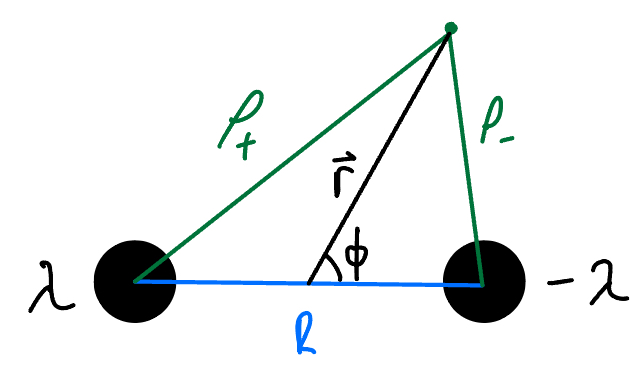
\includegraphics[width=0.5\textwidth]{prob2a.jpeg}
    \caption{Sketch of the problem setup [part (a)] transverse to two thin, long wires separated by distance $R$.}
    \label{fig:prob2a}
\end{figure}

\sol{

The potential a distance $\rho$ from a line charge with linear charge density $\lambda$ is
\begin{eqnarray}
    \Phi = \frac{\lambda}{2 \pi \epsilon_0} \ln{\Big( \frac{\rho_0}{\rho} \Big)} 
,\end{eqnarray}
where $\rho_0$ is some reference distance from the line charge where $\Phi = 0$.
The potential of a configuration of two parallel, oppositely charged lines is just
\begin{eqnarray}
    \Phi = \Phi_{+} + \Phi_{-} = \frac{\lambda}{2 \pi \epsilon_0} \ln{ \Big( \frac{\rho_{-}}{\rho_{+}} \Big) }
,\end{eqnarray}
where $\rho_{\pm}$ is just the distance between the point at which the potential is being evaluated and the line with charge per unit length $\pm \lambda$.
Notice that the dependence on $\rho_0$ cancels.
If we set up our coordinate system as in \fref{prob2a}, then we can express
\begin{eqnarray}
    \rho_{\pm} = \sqrt{ \Big( \frac{R}{2} \Big)^2 + r^2 \pm 2 \Big( \frac{R}{2} \Big) r \cos{\phi}}
\end{eqnarray}
via the law of cosines.
Hence, the potential in our coordinate system is
\begin{eqnarray}
    \Phi = \frac{\lambda}{4 \pi \epsilon_0} \ln{ \Big( \frac{R^2 + 4 r^2 - 4 R r \cos{\phi}}{R^2 + 4 r^2 + 4 R r \cos{\phi} } \Big) }
.\end{eqnarray}
On the surface of constant potential $\Phi = V$ we have
\begin{gather}
        e^{ 4 \pi \epsilon_0 V / \lambda } = \frac{R^2 + 4 r^2 - 4 R r \cos{\phi}}{R^2 + 4 r^2 + 4 R r \cos{\phi}} \\
        a(R^2 + 4r^2 + 4 R r \cos{\phi}) = R^2 + 4 r^2 - 4 R r \cos{\phi} \\
        (a - 1) R^2 + 4(a - 1) r^2 + 4(a + 1) R r \cos{\phi} = 0
\end{gather}
where we have denoted $a = \exp(4 \pi \epsilon_0 V / \lambda)$.
It is difficult to see a resemblance to any familiar surface in this form, so let us transform back into Cartesian coordinates, where $x = r \cos{\phi}$ and $y = r \sin{\phi}$:
\begin{gather}
    (a - 1) R^2 + 4(a - 1) (x^2 + y^2) + 4(a + 1) R x = 0 \\
    x^2 + \frac{a + 1}{a-1}Rx + y^2 = - \frac{R^2}{4} \\
    \Big[ x + \frac{a+1}{a-1} \frac{R}{2} \Big]^2 + y^2 = - \frac{R^2}{4} + \Big(\frac{a+1}{a - 1} \Big)^2  \frac{R^2}{4} \\
    \Big[ x + \coth{\Big( \frac{2 \pi \epsilon_0 V}{\lambda} \Big)} \frac{R}{2} \Big]^2 + y^2 = \Big[ \coth^2{\Big( \frac{2 \pi \epsilon_0 V}{\lambda} \Big)} - 1 \Big] \Big( \frac{R}{2} \Big)^2 \\
    \Big[ x + \coth{\Big( \frac{2 \pi \epsilon_0 V}{\lambda} \Big)} \frac{R}{2} \Big]^2 + y^2 = \frac{(R/2)^2}{\sinh^2{( 2 \pi \epsilon_0 V / \lambda ) }}
.\end{gather}
This is just the equation of a circle with center $(-\coth{(2 \pi \epsilon_0 V / \lambda)} [R / 2], 0)$ and radius $(R/2)/|\sinh{(2 \pi \epsilon_0 V / \lambda)}|$.
Notice that if $V > 0$ the center of this circle is always on the left of the line charge with linear density $+ \lambda$, while it is on the right of the line charge with linear density $-\lambda$ if $V < 0$.
Of course, the equipotential surface is a cylinder since the problem is translation invariant parallel to the lines.

(b) The capacitance of a setup with two conductors, one with charge $Q$ and the other with charge $-Q$, is just $C = Q/V$, where $V$ is the potential difference between the conductors.
The capacitance per unit length is then $C/L = \lambda/V$.
In this problem, we have two cylinderical conductors, with radii $a$ and $b$, respectively.
Without loss of generality, suppose that the conductor with radius $a$ has charge $+Q$ and therefore is at potential $V_{+}$, while the conductor with radius $b$ has charge $-Q$ and therefore is at potential $V_{-}$.
The potential difference $V = V_{+} - V_{-}$.

We can treat the potential on these surfaces as being set up by two line charges separated by some distance $R$.
We can then write
\begin{eqnarray}
    \label{eq:d}
    d = -\coth{\Big( \frac{2 \pi \epsilon_0 V_{-}}{\lambda} \Big)} + \coth{ \Big( \frac{2 \pi \epsilon_0 V_{+}}{\lambda} \Big) }
.\end{eqnarray}
Furthermore,
\begin{eqnarray}
    a = \frac{R}{2 \sinh{(2 \pi \epsilon_0 V_{+}} / \lambda)} ~{\rm and}~ b = -\frac{R}{2 \sinh{(2 \pi \epsilon_0 V_{-} / \lambda)}}
.\end{eqnarray}
We need to figure out $V_{+}$ and $V_{-}$ from these three equations (or at least their difference).

At the moment of this writing, divine inspiration has not struck in order to derive \eref{cap-per} \textit{a priori}, with only the equations above.
We proceed, taking direct guidance from the form of $C/L$.
Observe (letting $x_{\pm} = 2 \pi \epsilon_0 V_{\pm} / \lambda$)
\begin{align}
    d^2 - a^2 - b^2 &= \frac{R^2 (e^{2x_{+}} + e^{2 x_{-}})}{e^{2x_{+}} + e^{2x_{-}} - e^{2(x_{+}+x_{-})} - 1} \\
    2ab &= -\frac{2 R^2 e^{x_{+} + x_{-}}}{e^{2(x_{+} + x_{-})} - e^{2x_{+}} - e^{2x_{-}} - 1}
.\end{align}
Taking the ratio, we find
\begin{eqnarray}
    \begin{aligned}
        \frac{d^2 - a^2 - b^2}{2ab} &= \frac{e^{x_{+} - x_{-}} + e^{-(x_{+} - x_{-})}}{2} = \cosh{(x_{+} - x_{-})} \\
                                    &\Rightarrow V_{+} - V_{-} = \frac{\lambda}{2 \pi \epsilon_0} \cosh^{-1}{\Big( \frac{d^2 - a^2 - b^2}{2ab} \Big)} \\
                                    &\Rightarrow \eqbox{ \frac{C}{L} = \frac{2 \pi \epsilon_0}{\cosh^{-1}{(\frac{d^2 - a^2 - b^2}{2 a b})}} }
    .\end{aligned}
\end{eqnarray}

(c) The result of problem 1.7 is
\begin{eqnarray}
    \frac{C}{L} \approx \frac{2\pi \epsilon_0}{\ln(d^2/ab)}
.\end{eqnarray}
This is derived assuming $d \gg a,b$.
First, notice that $\cosh^{-1}{x} = \ln{(x + \sqrt{x^2 - 1})}$.
If $x$ is large, then $\cosh^{-1}{x} = \ln{(2x)}$
\begin{eqnarray}
    \cosh^{-1}{\Big( \frac{d^2 - a^2 - b^2}{2ab} \Big)} \approx \cosh^{-1}{\Big( \frac{d^2}{2ab} \Big)} \approx \ln{\Big( \frac{d^2}{ab} \Big)}
\end{eqnarray}
as desired.

We can determine the next non-vanishing power correction in $a/d$ and $b/d$ as follows.
Note that we can write
\begin{eqnarray}
    \begin{aligned}
        \cosh^{-1}{\Big( \frac{d^2}{2ab} \Big[ 1 - \frac{a^2 + b^2}{d^2} \Big] \Big)} &\approx \ln{\Big( \frac{d^2}{ab} \Big)} + \ln{\Big( 1 - \frac{a^2 + b^2}{d^2} \Big)} \\
                                                                                      &\approx \ln(\frac{d^2}{ab}) - \frac{a^2 + b^2}{d^2}
    \end{aligned}
,\end{eqnarray}
and therefore
\begin{eqnarray}
    \eqbox{
    \begin{aligned}
        \frac{C}{L} &\approx \frac{2 \pi \epsilon_0}{\ln(d^2/ab)} \Big[ 1 - \frac{a^2 + b^2}{ \ln(d^2/ab) d^2} \Big]^{-1} \\
                    &\approx \frac{2 \pi \epsilon_0}{\ln(d^2/ab)} \Big[ 1 + \frac{a^2 + b^2}{\ln(d^2/ab) d^2} \Big]
    \end{aligned}
}
\end{eqnarray}
at next-to-leading order in $a/d$ and $b/d$.

(d) Finally, if we have one cylinder inside the other such that $d < |a - b|$, then the capacitance per unit length is just
\begin{eqnarray}
    \frac{C}{L} = \frac{2 \pi \epsilon_0}{\cosh^{-1}(\frac{a^2 + b^2 - d^2}{2 a b})}
.\end{eqnarray}
This can be seen quite easily by taking $b \rightarrow -b$, which is done since $V_{-}$ is positive\footnote{We can say this since $V_{+}$ and $V_{-}$ are of the same sign and we can always shift the potential in such a way to make this true.}, and carrying out a similar set of manipulations as in part (b).

We can perform the sanity check for $d = 0$, which gives
\begin{eqnarray}
    \begin{aligned}
        \frac{C}{L} &= \frac{2 \pi \epsilon_0}{\cosh^{-1}(\frac{a^2 + b^2}{2ab})} = \frac{2 \pi \epsilon_0}{\ln(\frac{a^2 + b^2}{2ab} + \sqrt{\frac{a^{4} + 2 a^2 b^2 + b^{4}}{4 a^2 b^2} - 1})} \\
                    &= \frac{2 \pi \epsilon_0}{\ln(\frac{a^2 + b^2}{2ab} + \frac{a^2 - b^2}{2ab})} = \eqbox{ \frac{2 \pi \epsilon_0}{\ln(a/b)} }
    \end{aligned}
\end{eqnarray}
as derived in a previous homework.

}


\prob{3}{

An insulated, spherical, conducting shell of radius $a$ is in a uniform electric field $E_0$.
If the sphere is cut into two hemispheres by a plane perpendicular to the field, find the force required to prevent the hemispheres from separating \\[1pt]

(a) if the shell is uncharged;

(b) if the total charge on the shell is $Q$.

}

\begin{figure}[h!]
   \centering
   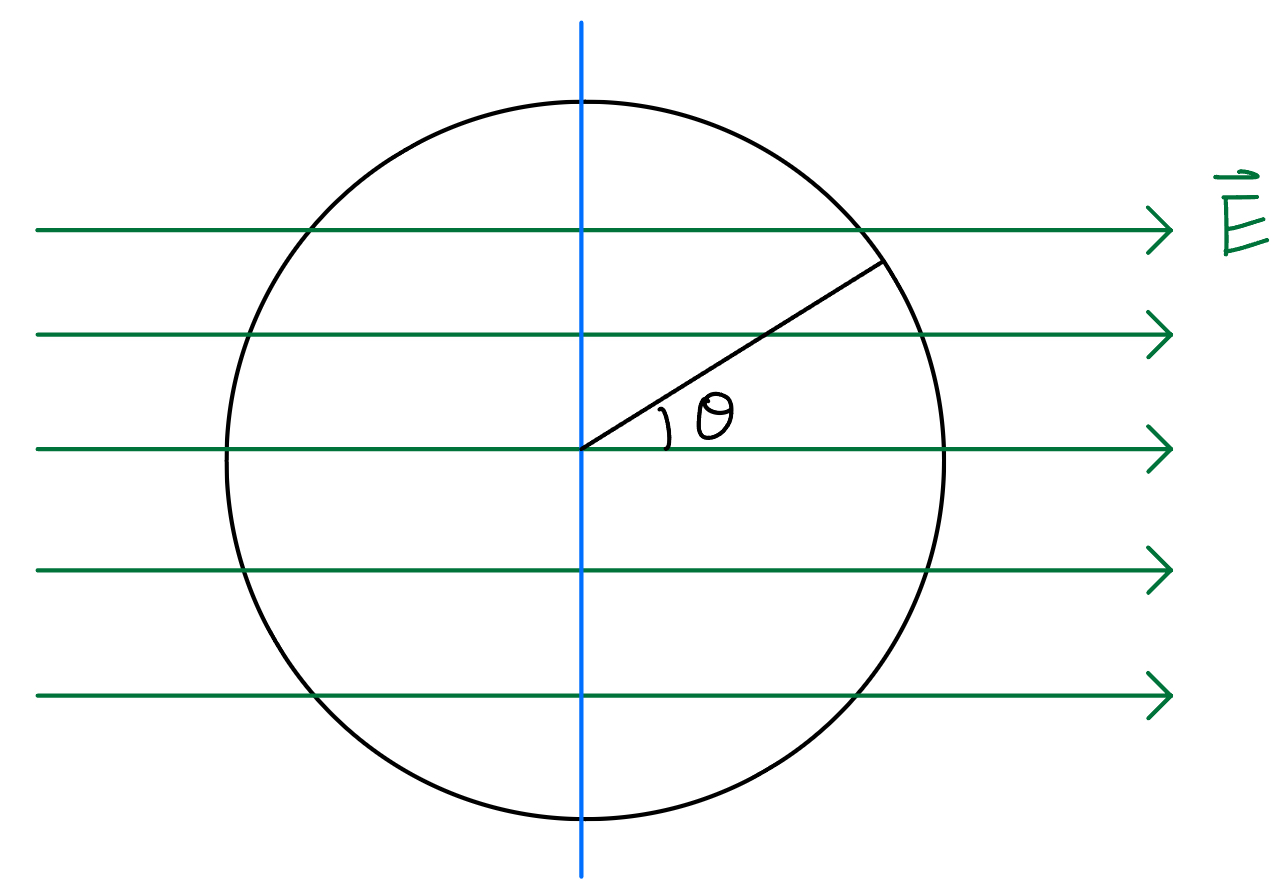
\includegraphics[width=0.4\textwidth]{prob3.jpeg}
   \caption{Insulated sphere immersed in constant electric magnetic field $\va*{E} = E_0 \vu*{z}$. Note that the electric field drawn is only the ambient field from before the insertion of the insulating sphere, not the electric field of the entire setup, which certainly is different because of the electric field set up by the induced surface charge density in parts (a)--(b) and also the charge $Q$ on the sphere in part (b).}
   \label{fig:prob3}
\end{figure}

\sol{

(a) The surface charge density induced by the uniform electric field is given as
\begin{eqnarray}
    \sigma = 3 \epsilon_0 E_0 \cos{\theta} 
,\end{eqnarray}
where $\theta$ is the angle relative to the direction of the direction of the electric field.
The force between on the right hemisphere is then
\begin{eqnarray}
\begin{aligned}
    \va*{F} &= \int_{S} \sigma \va*{E} \dd{S} = \int_{S} \frac{\sigma^2}{2 \epsilon_0} \vu*{r} \dd{S} \\
            &= \frac{9 \epsilon_0 E_0^2 a^2}{2} \int_{0}^{2 \pi} \int_{0}^{\pi/2} \cos^2{\theta} (\sin{\theta} \cos{\phi} \vu*{x} + \sin{\phi}\sin{\theta} \vu*{y} + \cos{\theta} \vu*{z}) \sin{\theta} \dd{\theta} \dd{\phi} \\
            &= 9 \pi \epsilon_0 E_0^2 a^2 \vu*{z} \int_{0}^{1} \cos^3{\theta} \dd{(\cos{\theta})} = \frac{9 \pi \epsilon_0 E_0^2 a^2}{4} \vu*{z}
.\end{aligned}
\end{eqnarray}
Hence, to oppose the force on the right hemisphere from the left, one must apply a force of the same magnitude in the opposite direction:
\begin{eqnarray}
    \eqbox{ \va*{F} = - \frac{9 \pi \epsilon_0 E_0^2 a^2}{4} \vu*{z} }
.\end{eqnarray}


(b) If the total charge on the shell is $Q$, then the total surface charge density is
\begin{eqnarray}
    \sigma = 3 \epsilon_0 E_0 \cos{\theta} + \frac{Q}{4 \pi a^2}
,\end{eqnarray}
and therefore
\begin{eqnarray}
    \begin{aligned}
        F &= \frac{\pi a^2}{2 \epsilon_0} \int_{0}^{1} \Big( 3 \epsilon_0 E_0 \cos{\theta} + \frac{Q}{4 \pi a^2} \Big)^2 \cos{\theta} \dd{(\cos{\theta})} \\
          &= \frac{9 \pi \epsilon_0 E_0^2 a^2}{4} + E_0 \frac{Q}{2} + \frac{Q^2}{32 \pi a^2}
    .\end{aligned}
\end{eqnarray}
Notice that this is not quite the force separating the two hemispheres, though.
The middle term is just the force from the constant electric field on the charge $Q/2$ in the right hemisphere.
This force is also present on the other hemisphere, meaning that the force one would have to apply to keep the right hemisphere attached to the left is
\begin{eqnarray}
    \eqbox{ \va*{F} = - \Big[ \frac{9 \pi \epsilon_0 E_0^2 a^2}{4} + \frac{Q^2}{32 \pi a^2} \Big] \vu*{z} }
.\end{eqnarray}


}




\end{document}
